\section{TINJAUAN PUSTAKA}

% Ubah konten-konten berikut sesuai dengan isi dari tinjauan pustaka
\subsection{Penelitian Terkait}
\begin{figure} [ht] \centering
    % Nama dari file gambar yang diinputkan
    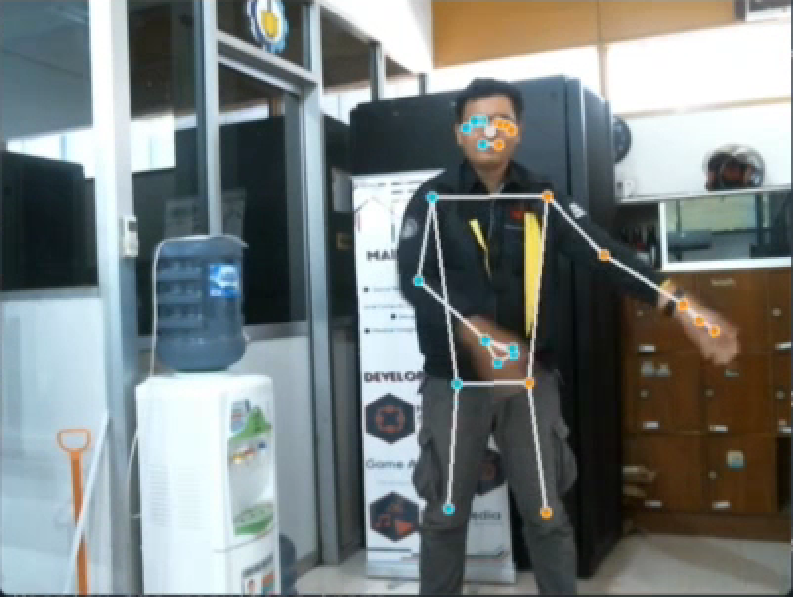
\includegraphics[scale=0.7]{gambar/contoh.png}
    % Keterangan gambar yang diinputkan
    \caption{Hasil Ujicoba Sementara}
    % Label referensi dari gambar yang diinputkan
    \label{fig:Ujicoba Sementara}
  \end{figure}
Berdasarkan Penelitian yang sudah dilakukan H. Y. Chang yang berjudul "Semaphore Flag Recognition Using Convolutional Neural Network" , Telah dilakukan ujicoba menggunakan Metode Convolutional Neural Network untuk membuat sistem identifikasi pose bendera semaphore . Sejauh ini penelitian yang dilakukan menggunakan citra gambar , Untuk Penelitian ini kami memanfaatkan fitur skeleton didalam MediaPipe 

\subsection{Teori/Konsep Dasar}

\subsubsection{Deep Learning}

% Contoh penggunaan referensi dari pustaka
Deep learning adalah sebuah metode dalam ilmu komputer yang menggunakan jaringan saraf tiruan yang terdiri dari banyak lapisan untuk memproses data dan mengekstrak fitur yang berguna dari data tersebut. Jaringan saraf tiruan ini dapat diaplikasikan pada berbagai macam tugas, termasuk pengenalan wajah, pengenalan suara, dan pemrosesan bahasa alami.

Deep learning telah menjadi salah satu teknik terpenting dalam bidang pembelajaran mesin dan telah menghasilkan hasil yang luar biasa dalam berbagai aplikasi, termasuk pengenalan wajah, pengenalan suara, dan pemrosesan bahasa alami.

Saat ini Deep Learning sudah diterapkan di berbagai bidang seperti di bidang pemasaran , Deep learning dapat digunakan dalam pemasaran untuk memprediksi keputusan pembelian pelanggan atau menyarankan produk yang mungkin akan diminati pelanggan berdasarkan data sebelumnya. Lalu juga ada di bidang kesehatan seperti  menganalisis data pasien dan mengidentifikasi pola yang dapat membantu dokter mengdiagnosis penyakit dan memberikan perawatan yang tepat . Dan masih banyak lagi berbagai macam implementasi Deep Learning di berbagai bidang dalam kehidupan manusia 

\subsubsection{CNN / Convolutional Neural Network}
Convolutional Neural Network (CNN) adalah sebuah jaringan saraf tiruan yang dapat digunakan untuk mengolah data yang memiliki struktur spasial, seperti gambar atau video. CNN terdiri dari lapisan-lapisan yang terdiri dari neuron-neuron yang terhubung dengan bobot dan bias. Setiap lapisan dapat menerima input dari lapisan sebelumnya dan menghasilkan output ke lapisan selanjutnya.

CNN menggunakan operasi konvolusi untuk memproses data yang memiliki struktur spasial. Konvolusi adalah sebuah operasi matematis yang menggunakan filter untuk mengambil fitur dari data. Filter ini dapat berupa matriks dengan bobot yang dapat dilatih selama proses pembelajaran. Konvolusi memungkinkan CNN untuk mengekstrak fitur yang berguna dari data yang memiliki struktur spasial seperti gambar atau video.

\subsubsection{Bendera Semaphore}
Bendera Semaphore adalah sebuah sistem komunikasi yang menggunakan posisi dari dua bendera untuk mengirimkan pesan. Bendera Semaphore pertama kali dikembangkan pada abad ke-18 oleh seorang ahli matematika Prancis bernama Claude Chappe sebagai cara untuk mengirimkan pesan telegraf tanpa menggunakan kabel.

Bendera Semaphore menggunakan dua bendera yang dapat digerakkan ke posisi yang berbeda, yang masing-masing mewakili sebuah huruf dari alfabet atau angka. Setiap posisi bendera menunjukkan sebuah karakter yang dapat ditransmisikan kepada penerima pesan. Bendera Semaphore biasanya digunakan untuk mengirimkan pesan jarak jauh, misalnya antar kapal atau antar kota.